% Created by tikzDevice version 0.10.1 on 2016-02-27 13:16:47
% !TEX encoding = UTF-8 Unicode
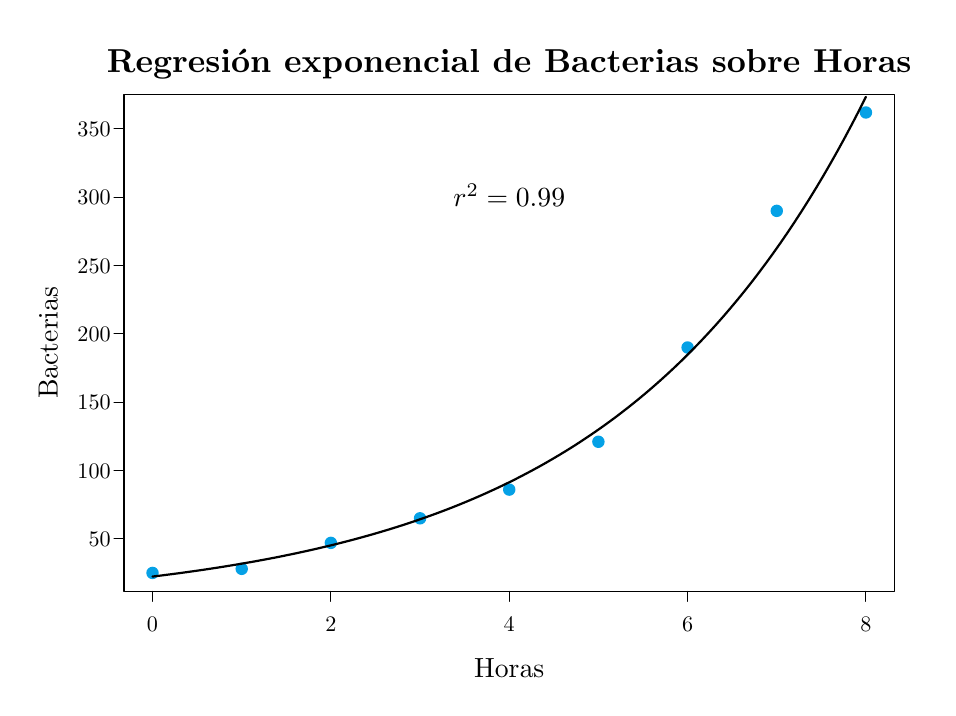
\begin{tikzpicture}[x=1pt,y=1pt]
\definecolor{fillColor}{RGB}{255,255,255}
\path[use as bounding box,fill=fillColor,fill opacity=0.00] (0,0) rectangle (325.21,238.49);
\begin{scope}
\path[clip] ( 34.80, 34.80) rectangle (313.21,214.49);
\definecolor{fillColor}{RGB}{5,161,230}

\path[fill=fillColor] ( 45.11, 41.46) circle (  2.25);

\path[fill=fillColor] ( 77.34, 42.94) circle (  2.25);

\path[fill=fillColor] (109.56, 52.32) circle (  2.25);

\path[fill=fillColor] (141.78, 61.20) circle (  2.25);

\path[fill=fillColor] (174.01, 71.57) circle (  2.25);

\path[fill=fillColor] (206.23, 88.85) circle (  2.25);

\path[fill=fillColor] (238.46,122.92) circle (  2.25);

\path[fill=fillColor] (270.68,172.29) circle (  2.25);

\path[fill=fillColor] (302.90,207.84) circle (  2.25);
\end{scope}
\begin{scope}
\path[clip] (  0.00,  0.00) rectangle (325.21,238.49);
\definecolor{drawColor}{RGB}{0,0,0}

\path[draw=drawColor,line width= 0.4pt,line join=round,line cap=round] ( 45.11, 34.80) -- (302.90, 34.80);

\path[draw=drawColor,line width= 0.4pt,line join=round,line cap=round] ( 45.11, 34.80) -- ( 45.11, 31.21);

\path[draw=drawColor,line width= 0.4pt,line join=round,line cap=round] (109.56, 34.80) -- (109.56, 31.21);

\path[draw=drawColor,line width= 0.4pt,line join=round,line cap=round] (174.01, 34.80) -- (174.01, 31.21);

\path[draw=drawColor,line width= 0.4pt,line join=round,line cap=round] (238.46, 34.80) -- (238.46, 31.21);

\path[draw=drawColor,line width= 0.4pt,line join=round,line cap=round] (302.90, 34.80) -- (302.90, 31.21);

\node[text=drawColor,anchor=base,inner sep=0pt, outer sep=0pt, scale=  0.80] at ( 45.11, 20.40) {0};

\node[text=drawColor,anchor=base,inner sep=0pt, outer sep=0pt, scale=  0.80] at (109.56, 20.40) {2};

\node[text=drawColor,anchor=base,inner sep=0pt, outer sep=0pt, scale=  0.80] at (174.01, 20.40) {4};

\node[text=drawColor,anchor=base,inner sep=0pt, outer sep=0pt, scale=  0.80] at (238.46, 20.40) {6};

\node[text=drawColor,anchor=base,inner sep=0pt, outer sep=0pt, scale=  0.80] at (302.90, 20.40) {8};

\path[draw=drawColor,line width= 0.4pt,line join=round,line cap=round] ( 34.80, 53.80) -- ( 34.80,201.91);

\path[draw=drawColor,line width= 0.4pt,line join=round,line cap=round] ( 34.80, 53.80) -- ( 31.21, 53.80);

\path[draw=drawColor,line width= 0.4pt,line join=round,line cap=round] ( 34.80, 78.48) -- ( 31.21, 78.48);

\path[draw=drawColor,line width= 0.4pt,line join=round,line cap=round] ( 34.80,103.17) -- ( 31.21,103.17);

\path[draw=drawColor,line width= 0.4pt,line join=round,line cap=round] ( 34.80,127.85) -- ( 31.21,127.85);

\path[draw=drawColor,line width= 0.4pt,line join=round,line cap=round] ( 34.80,152.54) -- ( 31.21,152.54);

\path[draw=drawColor,line width= 0.4pt,line join=round,line cap=round] ( 34.80,177.23) -- ( 31.21,177.23);

\path[draw=drawColor,line width= 0.4pt,line join=round,line cap=round] ( 34.80,201.91) -- ( 31.21,201.91);

\node[text=drawColor,anchor=base east,inner sep=0pt, outer sep=0pt, scale=  0.80] at ( 30.00, 51.04) {50};

\node[text=drawColor,anchor=base east,inner sep=0pt, outer sep=0pt, scale=  0.80] at ( 30.00, 75.73) {100};

\node[text=drawColor,anchor=base east,inner sep=0pt, outer sep=0pt, scale=  0.80] at ( 30.00,100.41) {150};

\node[text=drawColor,anchor=base east,inner sep=0pt, outer sep=0pt, scale=  0.80] at ( 30.00,125.10) {200};

\node[text=drawColor,anchor=base east,inner sep=0pt, outer sep=0pt, scale=  0.80] at ( 30.00,149.78) {250};

\node[text=drawColor,anchor=base east,inner sep=0pt, outer sep=0pt, scale=  0.80] at ( 30.00,174.47) {300};

\node[text=drawColor,anchor=base east,inner sep=0pt, outer sep=0pt, scale=  0.80] at ( 30.00,199.16) {350};

\path[draw=drawColor,line width= 0.4pt,line join=round,line cap=round] ( 34.80, 34.80) --
	(313.21, 34.80) --
	(313.21,214.49) --
	( 34.80,214.49) --
	( 34.80, 34.80);
\end{scope}
\begin{scope}
\path[clip] (  0.00,  0.00) rectangle (325.21,238.49);
\definecolor{drawColor}{RGB}{0,0,0}

\node[text=drawColor,anchor=base,inner sep=0pt, outer sep=0pt, scale=  1.20] at (174.01,222.30) {\bfseries Regresión exponencial de Bacterias sobre Horas};

\node[text=drawColor,anchor=base,inner sep=0pt, outer sep=0pt, scale=  1.00] at (174.01,  3.60) {Horas};

\node[text=drawColor,rotate= 90.00,anchor=base,inner sep=0pt, outer sep=0pt, scale=  1.00] at ( 10.80,124.65) {Bacterias};
\end{scope}
\begin{scope}
\path[clip] ( 34.80, 34.80) rectangle (313.21,214.49);
\definecolor{drawColor}{RGB}{0,0,0}

\path[draw=drawColor,line width= 0.8pt,line join=round,line cap=round] ( 45.11, 40.15) --
	( 47.69, 40.46) --
	( 50.27, 40.79) --
	( 52.85, 41.12) --
	( 55.42, 41.46) --
	( 58.00, 41.82) --
	( 60.58, 42.18) --
	( 63.16, 42.55) --
	( 65.73, 42.94) --
	( 68.31, 43.33) --
	( 70.89, 43.74) --
	( 73.47, 44.16) --
	( 76.05, 44.59) --
	( 78.62, 45.03) --
	( 81.20, 45.48) --
	( 83.78, 45.95) --
	( 86.36, 46.43) --
	( 88.94, 46.92) --
	( 91.51, 47.43) --
	( 94.09, 47.96) --
	( 96.67, 48.49) --
	( 99.25, 49.05) --
	(101.83, 49.62) --
	(104.40, 50.20) --
	(106.98, 50.81) --
	(109.56, 51.42) --
	(112.14, 52.06) --
	(114.72, 52.72) --
	(117.29, 53.39) --
	(119.87, 54.09) --
	(122.45, 54.80) --
	(125.03, 55.53) --
	(127.60, 56.29) --
	(130.18, 57.06) --
	(132.76, 57.86) --
	(135.34, 58.68) --
	(137.92, 59.53) --
	(140.49, 60.39) --
	(143.07, 61.29) --
	(145.65, 62.21) --
	(148.23, 63.15) --
	(150.81, 64.12) --
	(153.38, 65.12) --
	(155.96, 66.15) --
	(158.54, 67.21) --
	(161.12, 68.30) --
	(163.70, 69.42) --
	(166.27, 70.57) --
	(168.85, 71.75) --
	(171.43, 72.97) --
	(174.01, 74.22) --
	(176.59, 75.51) --
	(179.16, 76.84) --
	(181.74, 78.20) --
	(184.32, 79.60) --
	(186.90, 81.04) --
	(189.47, 82.53) --
	(192.05, 84.05) --
	(194.63, 85.62) --
	(197.21, 87.23) --
	(199.79, 88.89) --
	(202.36, 90.60) --
	(204.94, 92.36) --
	(207.52, 94.16) --
	(210.10, 96.02) --
	(212.68, 97.93) --
	(215.25, 99.90) --
	(217.83,101.92) --
	(220.41,104.00) --
	(222.99,106.14) --
	(225.57,108.34) --
	(228.14,110.60) --
	(230.72,112.93) --
	(233.30,115.32) --
	(235.88,117.78) --
	(238.46,120.32) --
	(241.03,122.92) --
	(243.61,125.60) --
	(246.19,128.36) --
	(248.77,131.19) --
	(251.34,134.10) --
	(253.92,137.10) --
	(256.50,140.19) --
	(259.08,143.36) --
	(261.66,146.62) --
	(264.23,149.98) --
	(266.81,153.43) --
	(269.39,156.98) --
	(271.97,160.63) --
	(274.55,164.39) --
	(277.12,168.25) --
	(279.70,172.23) --
	(282.28,176.31) --
	(284.86,180.52) --
	(287.44,184.84) --
	(290.01,189.29) --
	(292.59,193.86) --
	(295.17,198.57) --
	(297.75,203.41) --
	(300.33,208.39) --
	(302.90,213.51);

\node[text=drawColor,anchor=base,inner sep=0pt, outer sep=0pt, scale=  1.00] at (174.01,173.76) {$r^2=0.99$};
\end{scope}
\end{tikzpicture}
